\section{Functional role of classes}
\label{sec:functional-role}

\subsection{Java Transaction Service}
The two classes which are assigned to us are part of the Java Transaction Service (JTS) implementation by Sun.
By Wikipedia\footnote{\url{https://en.wikipedia.org/wiki/Java_transaction_service}}:
\begin{quote}
The \textbf{Java Transaction Service (JTS)} is a specification for building a transaction manager that maps onto the Object Management Group (OMG) Object Transaction Service (OTS) used in the Common Object Request Broker Architecture (CORBA) architecture. It uses General Inter-ORB Protocol (IIOP) to propagate the transactions between multiple JTS transaction managers.
\end{quote}

The complete specification of Java Transaction Service is available on Oracle's website~\cite{jts-specification} and defines JTS as follows:
\begin{quotation}
This is the Java Transaction Service (JTS) Specification.
JTS specifies the
implementation of a transaction manager which supports the JTA specification at
the high-level and implements the Java mapping of the OMG Object Transaction
Service (OTS) 1.1 Specification at the low-level.

JTS uses the CORBA OTS interfaces for interoperability and portability (that is, \textbf{CosTransactions} and CosTSPortability).
These interfaces define a standard mechanism for any implementation that utilizes IIOP (Internet InterORB Protocol) to generate and
propagate transaction context between JTS Transaction Managers. Note, this also
permits the use of other API over the IIOP transport mechanism to be used; for
example, RMI over IIOP is allowed.
\end{quotation}

\begin{figure}[h]
\centering
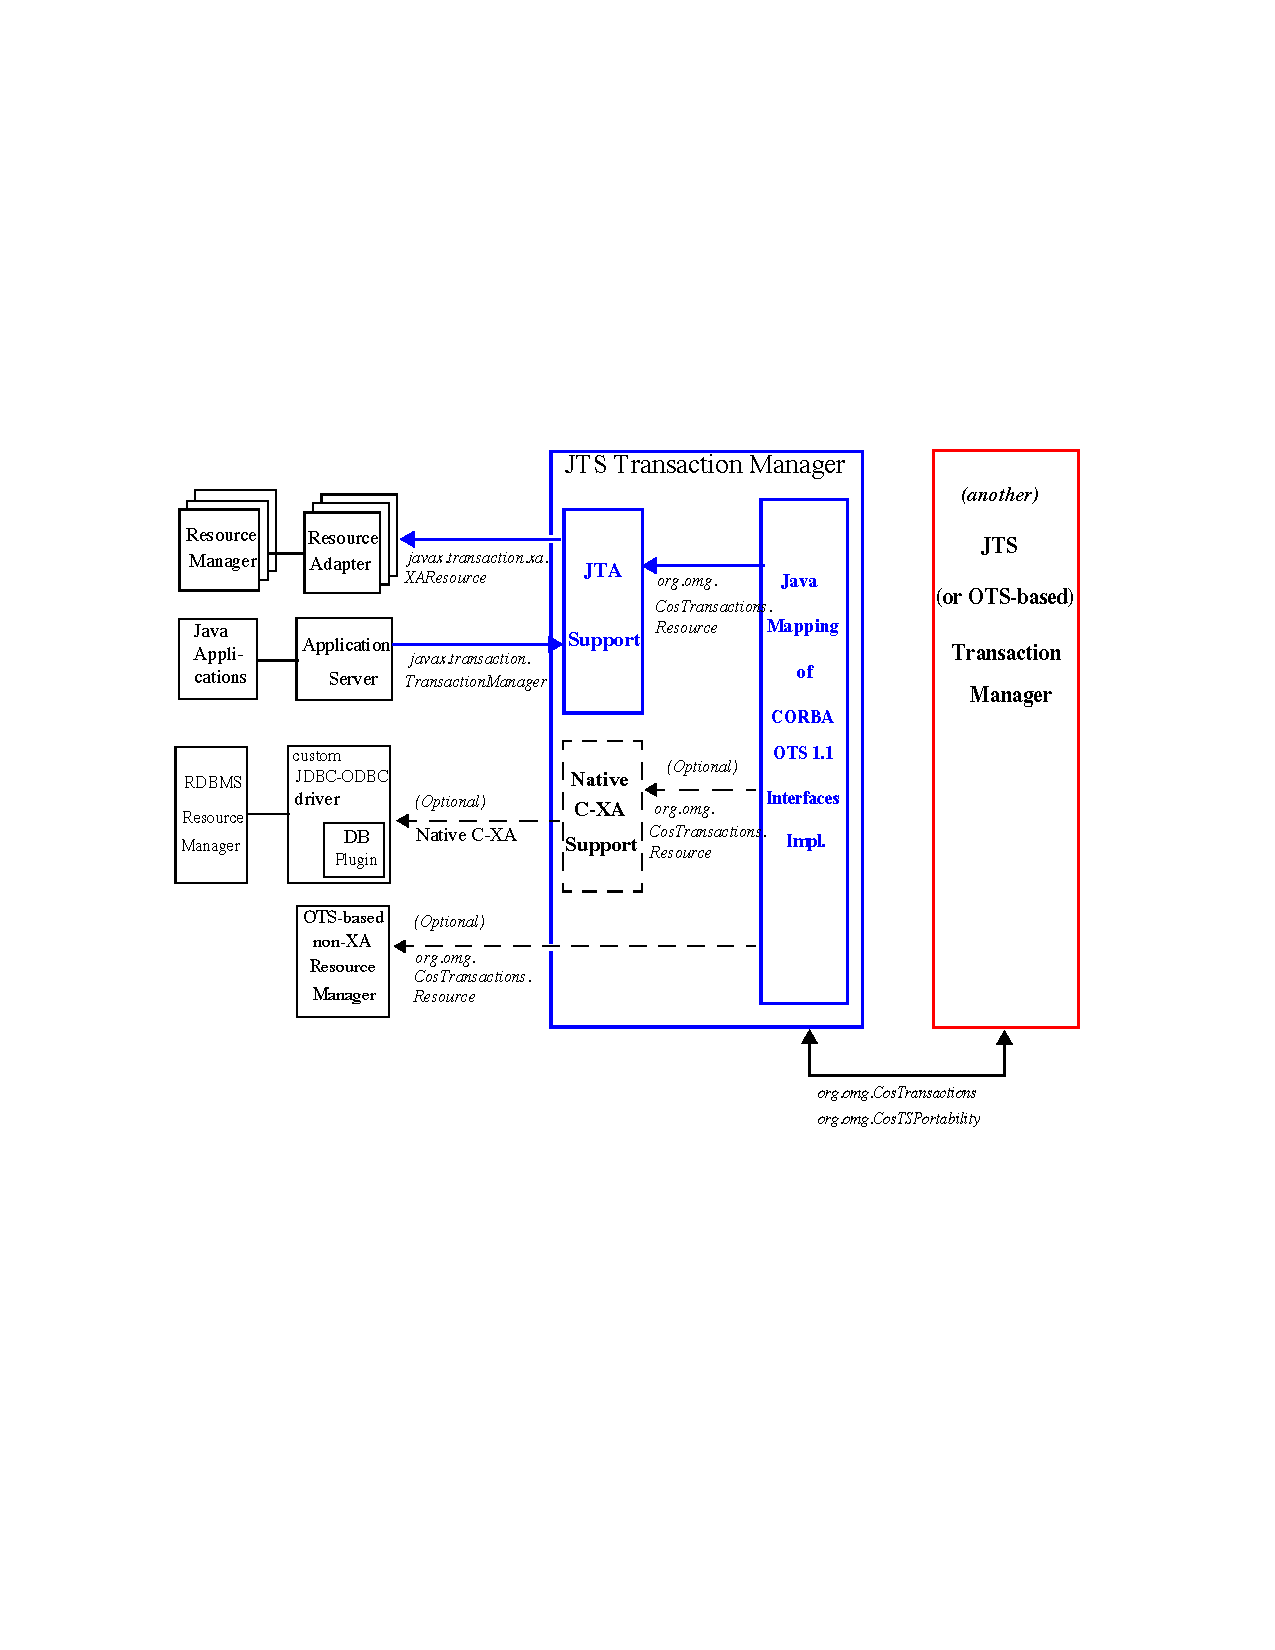
\includegraphics[width=\textwidth]{figures/JTSDiagram}
\caption{This figure is taken from the JTS specification and shows the implementation of a JTS Transaction Manager.}
\end{figure}

\subsection{CosTransactions package}
% TODO

\subsection{CoordinatorLog class}
% TODO

\subsection{RecoveryManager class}
% TODO
